\section{Methodology}
\label{sec:method}

\subsection{Datasets}

To ensure reliable and comparable results, four widely used benchmark datasets from the literature were selected at the beginning of this study. All datasets contain facial images categorized into the six target expressions: anger, disgust, fear, happiness, sadness, and surprise. The datasets employed were a smaller version of AffectNet \cite{affectnet} (22,629 images), CK+ \cite{ckplus}  (927 images), FER+ \cite{ferplus} (56,269 images), and RAF-DB \cite{rafdb} (12,135 images).

FER+ was chosen instead of the original FER2013 due to its improved labeling quality, which has a direct impact on model performance and reliability. Moreover, the selected datasets provide diversity in terms of age, ethnicity, and gender, which is essential for improving the generalization capability of the models. Although AffectNet, CK+, and FER+ include an additional \textit{contempt} label, this class was excluded from the experiments as it falls outside the scope of the present study. The data includes both grayscale and RGB images. Image formats vary between JPEG and PNG, which does not affect the preprocessing or training pipeline.

After the initial training sessions, the developed models exhibited strong overfitting. To mitigate this issue, additional datasets were sought, and access requests were submitted to multiple institutions worldwide to expand the training data.

At the end of the data collection process, a total of 310,215 facial images were gathered. In addition to the previously mentioned datasets, the final corpus also included images from EmoSet \cite{emoset}, JAFFE \cite{jaffe}, MMA-FEDB \cite{mma}, ExpWild \cite{expw} and WSEFEP \cite{wse-fep}. All datasets were carefully curated and harmonized to match the six target emotion categories used in this study.

Several challenges were encountered during dataset collection and curation. Some datasets contained incorrectly labeled samples, including statues, cartoon characters, or animals assigned to human emotion categories. In other cases, images were organized per subject rather than per emotion category, without consistent naming conventions, which prevented automated separation. Furthermore, some small datasets were ultimately discarded due to insufficient sample size or poor labeling quality.

As illustrated in the Figure \ref{fig:processed_images_distribution}, the aggregated datasets are imbalanced, with a significantly higher number of happiness samples compared to the other emotion categories.

\subsection{Cross-Dataset Generalization Strategy}

For the final training phase, CK+ and KDEF \cite{kdef} were deliberately excluded from the training set in order to evaluate the generalization capability of the proposed model on unseen datasets. It is important to emphasize that both datasets are relatively balanced.

KDEF contains high-quality, well-controlled facial images captured under consistent lighting and pose conditions, including photos from multiple angles up to 90º. This increased variation in viewpoint makes it more challenging for our models to accurately predict the expressions, which explains their lower performance on KDEF.

By excluding CK+ and KDEF from training, these datasets served as independent test sets, enabling a more rigorous evaluation of cross-dataset generalization performance.

\subsection{Data Pre-Processing Methodology}
The pre-processing pipeline functions as a sequential execution of image evaluation modules, where images failing specific quality thresholds are programmatically discarded. The evolution of this strategy transitioned from strict curation to selective filtering across two empirical phases.

\textbf{Phase 1: Aggressive Filtering for a Specialized Use Case}
The primary hypothesis for Phase 1 was that the model would perform optimally if trained exclusively on perfect, high-quality images that mirrored the target demonstration environment (a user looking directly into a high-quality camera). To enforce this pristine standard, the initial pipeline utilized all available filters sequentially:
\begin{itemize}
    \item \textbf{Lighting Filter:} Analyzed the mean pixel intensity and standard deviation, discarding images that were excessively dark, overly bright, or lacked sufficient contrast.
    \item \textbf{Blur Detection:} Assessed image sharpness using frequency analysis via a Fast Fourier Transform (FFT). Images lacking sufficient high-frequency components were rejected.
    \item \textbf{Roll Correction:} Evaluated the image across four rotational states ($0^{\circ}, 90^{\circ}, 180^{\circ}, 270^{\circ}$), selecting the orientation that yielded the highest face detection confidence.
    \item \textbf{Yaw Filtering:} RetinaFace detected the face, and 6DRepNet predicted the 3D pose. To guarantee a strict frontal viewpoint, any image with a yaw angle exceeding $45^{\circ}$ was discarded.
    \item \textbf{Conditional Cropping:} If the ratio of the face area to the total image area was less than $0.4$, indicating a small face with significant background, the image was cropped with proportional padding; otherwise, the original image was retained.
\end{itemize}
In Phase 1, we retained approximately 91,960 images after aggressive filtering.

\textbf{Phase 2: Resolving the Augmentation Contradiction}
The aggressively filtered dataset from Phase 1 caused the models to overfit rapidly. To combat this, data augmentation techniques were applied (adding artificial noise, altering brightness, introducing artificial blur, and utilizing MixUp).

This sequence exposed a fundamental contradiction: we were actively removing naturally difficult images during the pre-processing stage, only to artificially recreate those exact conditions during the augmentation stage. Furthermore, augmentations like MixUp produce overlapping visual structures that standard face detectors completely fail to recognize, meaning such images would be universally rejected by strict filters. Recognizing that the model required this data variance to generalize, Phase 2 drastically reduced the aggression of the filtering pipeline:
\begin{itemize}
    \item \textbf{Reduced Aggression:} The universal application of blur, yaw, roll, and lighting filters was halted. For high-quality datasets (AffectNet, CKplus, FERPlus, RAF-DB), the pipeline was stripped down to utilize only structural standardization.
    \item \textbf{Selective Cleaning:} Aggressive techniques were retained only for uncleaned, chaotic datasets (e.g., ExpW and EmoSet), which utilized the cropping module, face detection validation, and manual exclusion of specific emotion labels.
\end{itemize}
In Phase 2, we started with 310,215 images. After selective pre-processing, we retained 229,478 images.

\definecolor{darkblue}{RGB}{52, 73, 102}
\definecolor{steelblue}{RGB}{100, 130, 160}

\begin{figure}[h]
\centering
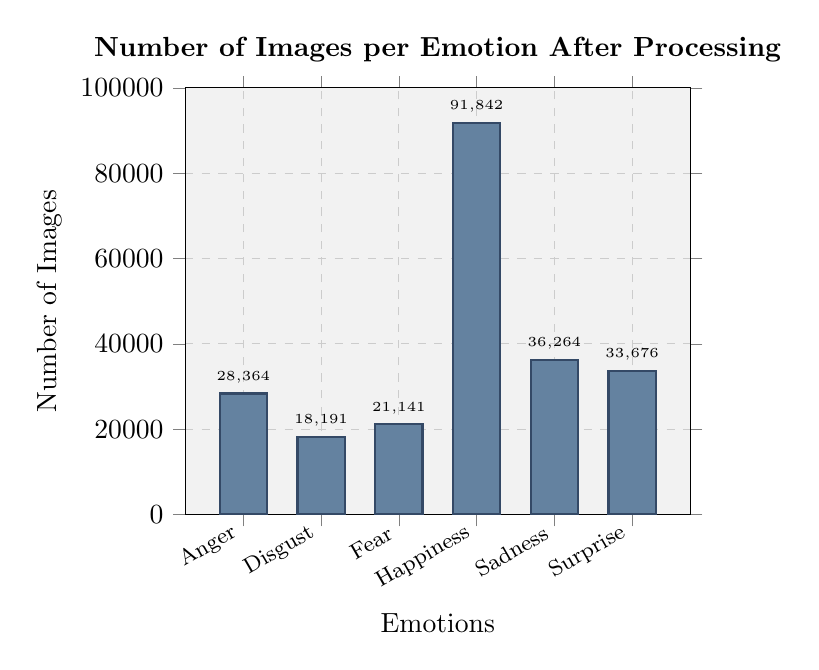
\begin{tikzpicture}
\begin{axis}[
    title={\textbf{Number of Images per Emotion After Processing}},
    ybar,
    bar width=0.6cm,
    width=8cm,
    height=7cm,
    symbolic x coords={Anger, Disgust, Fear, Happiness, Sadness, Surprise},
    xtick=data,
    x tick label style={rotate=30, anchor=east, font=\footnotesize},
    xlabel={Emotions},
    ylabel={Number of Images},
    ymin=0,
    ymax=100000,
    ytick={0,20000,40000,60000,80000,100000},
    scaled y ticks=false, 
    yticklabel style={/pgf/number format/fixed, /pgf/number format/1000 sep={}},
    nodes near coords,
    nodes near coords style={font=\tiny},
    every node near coord/.append style={
        /pgf/number format/fixed,
        /pgf/number format/precision=0
    },
    axis background/.style={fill=gray!10},
    grid=major,
    grid style={dashed, gray!40},
    tick align=outside,
    enlarge x limits=0.15,
]

\addplot[
    fill=steelblue,
    draw=darkblue,
    thick
] coordinates {
    (Anger,    28364)
    (Disgust,  18191)
    (Fear,     21141)
    (Happiness, 91842)
    (Sadness,  36264)
    (Surprise, 33676)
};

\end{axis}
\end{tikzpicture}
\caption{Number of Images per Emotion After Processing}
\label{fig:processed_images_distribution}
\end{figure}

\textbf{Standardization and Deduplication}
To finalize the datasets, all images underwent structural standardization:
\begin{itemize}
    \item \textbf{Channel Normalization:} All inputs were converted to a 3-channel RGB format to ensure consistent tensor depth.
    \item \textbf{Resizing:} Images were zero-padded to achieve a square aspect ratio and subsequently resized to exactly $64 \times 64$ pixels. We utilized cubic interpolation if the original image was smaller than $64 \times 64$.
    \item \textbf{Deduplication:} Duplicate or highly similar images were purged using a combination of perceptual hashing (pHash) and difference hashing (dHash) to ensure strict separation between training and validation distributions.
\end{itemize}

\textbf{Dataset Splitting}
At the beginning, we followed an 80\%/10\%/10\% split strategy, where 80\% of the data was used for training, 10\% for validation, and 10\% for testing.
Towards the end of the project, some of us adopted a 90\%/10\% split strategy in most experiments. The training set comprised 90\% of the data, while 10\% was reserved for validation (evaluation). For the final test set, we exclusively utilized two specific high-quality datasets: CK+ and KDEF. This rigorous separation ensured that our final performance metrics reflected true generalization on standardized benchmarks.

\subsection{Architectural Adaptations}

\subsubsection{Basic CNNs and ResNet18 models}
To ensure experimental comparability, two baseline convolutional neural networks (3-layer and 5-layer CNNs) were implemented alongside a modified version of ResNet-18, in which the initial $7 \times 7$ convolution was replaced with a $3 \times 3$ kernel and the input resolution was reduced from $224 \times 224$ to $64 \times 64$. 

\subsubsection{ResNet18 with Squeeze-and-Excitation}
Our model is based on ResNet18 and is extended with a squeeze-and-excitation (SE) attention module. ResNet18 serves as a stable baseline with moderate capacity (roughly 11--12 million parameters). Results from compact FER literature, including CERN, suggest that attention mechanisms can improve performance across different model sizes, supporting our use of SE as a low-overhead architectural enhancement \cite{GERA20229}.

The input to our network is a standardized RGB face image of size 64x64. Since this is much smaller than the standard ImageNet setting (224x224), we avoid the original ResNet stem (7x7 stride-2 convolution plus stride-2 max pooling), because it would reduce spatial resolution too early and remove fine facial details. Instead, we use a 3x3 convolution with stride 1 and omit early pooling to preserve spatial information \cite{cs231n2017}.

After the stem, we follow the standard ResNet18 design with four residual stages and stage-wise downsampling.

We augment the ResNet18 backbone with squeeze-and-excitation (SE) blocks, which perform lightweight channel-wise attention by learning per-channel scaling factors from globally pooled features, improving representational capacity with minimal overhead \cite{hu2018senet}. The motivation for using a lightweight attention mechanism is consistent with the goal of improving robustness without greatly increasing model size and is aligned with compact FER approaches such as CERN \cite{GERA20229}.
\subsection{Class Imbalance and Advanced Loss Functions}

A significant challenge encountered in our training pipeline is the severe class imbalance within our aggregated dataset, where the \textit{happiness} class constitutes approximately 40\% of the total data. Under standard cross-entropy loss, this imbalance introduces a fundamental bias where the majority class becomes the default, high-confidence prediction. This phenomenon is driven by two factors:
\begin{itemize}
    \item \textbf{Frequency versus Difficulty:} The \textit{happiness} class typically presents distinct visual markers (e.g., a smile) that are easily learned. Conversely, minority classes such as \textit{fear} and \textit{disgust} rely on subtle ocular and brow micro-expressions that degrade heavily at lower resolutions, such as $64 \times 64$ pixels.
    \item \textbf{Loss Gradients:} Because majority classes occur more frequently, they contribute a disproportionately large share of the gradient updates. The model minimizes the global objective simply by maximizing confidence in the frequent, easy classes, functionally neglecting the minority classes.
\end{itemize}

To address this imbalance without relying on a \texttt{WeightedRandomSampler}, we modified the training objective by evaluating two advanced loss functions:

\begin{itemize}
    \item \textbf{Class-Balanced Focal Loss (CB-FL):} This loss was applied to \textbf{both the ResNet18+SE and EfficientNetV2-S models}. It assigns larger weights to underrepresented classes using the effective number of samples \cite{cui2019classbalancedlossbasedeffective}, while the focal component reduces the contribution of well-classified (easy) samples so that the model continues learning from harder examples \cite{lin2018focallossdenseobject}.
    \item \textbf{Label-Distribution-Aware Margin Loss (LDAM) with Deferred Re-Weighting (DRW):} This loss was evaluated \textbf{exclusively on the EfficientNetV2-S model}. LDAM modifies the logit outputs by assigning a significantly larger mathematical margin to minority classes \cite{cao2019learning}. This strictly penalizes the model unless it maintains extreme confidence when predicting rare classes, thereby enforcing wider decision boundaries around them. The DRW strategy schedules the training such that the model trains without artificial weights for the initial epochs to learn robust feature representations. In the final epochs, strict class frequency weights are applied to fine-tune the decision boundaries for the minority classes without corrupting the initial feature learning phase.
\end{itemize}

\subsubsection{Alternative Architectures}
During the evaluation phase, three low-parameter architectures were tested to compare different modern deep learning paradigms. Adapting these models for $64 \times 64$ inputs required specific architectural modifications, primarily reducing spatial downsampling.

\begin{itemize}
    \item \textbf{Vim (Vision Mamba, $\sim$7M parameters):} Vim \cite{zhu2024visionmambaefficientvisual} was chosen because it is a novel model challenging standard Transformers by utilizing bidirectional State Space Models (SSMs), promising exceptionally low GPU memory usage. To adapt it for $64 \times 64$ images, the patch size was changed from $16 \times 16$ to $8 \times 8$ to provide a functional sequence length of 64 tokens.
    \item \textbf{CCT-7 (Compact Convolutional Transformer, $\sim$4M parameters):} CCT-7 \cite{hassani2022escapingbigdataparadigm} was selected to test a small Transformer specifically designed to handle small images by using a convolutional tokenizer instead of linear patch embeddings.
    \item \textbf{ConvNeXt V2 Atto ($\sim$3.7M parameters):} This model \cite{woo2023convnextv2codesigningscaling} was chosen to evaluate how a state-of-the-art pure Convolutional Neural Network operates in a constrained parameter regime. The original architecture features a stem convolution with a stride of 4. For a $64 \times 64$ image, this immediately shrinks the feature map to $16 \times 16$. The stem stride was explicitly changed to 1 to preserve spatial information.
\end{itemize}

\subsubsection{EfficientNetV2-S Adaptations}
EfficientNetV2-S \cite{tan2021efficientnetv2smallermodelsfaster} was selected for its MBConv blocks and Squeeze-and-Excitation (SE) attention, which effectively amplify emotional markers like micro-expressions while suppressing background noise.

\textbf{Architectural and Augmentation Adaptations}
To process $64 \times 64$ images effectively, two major pipeline adjustments were executed:
\begin{itemize}
    \item \textbf{Stem Stride Fix:} The original stem stride of 2 was reduced to 1. This modification preserved the full spatial resolution through the initial layers, preventing the immediate loss of fine facial details.
    \item \textbf{Minimized Destructive Augmentation:} Initial training with standard ImageNet settings (Mixup $\alpha=0.8$) obliterated facial features. We implemented a low-interference pipeline to minimize data destruction while maintaining regularization. This included reducing Mixup to 0.2, limiting CutMix to a maximum of 0.3, and using gentle affine transformations. This ensured that while the model was forced to reconstruct features, the core emotional signal remained intact.
\end{itemize}

\subsection{Explainable AI}

AI systems that only expose the input and output of the model to the user are called "black box models". The difficulty this design poses lies in the fact that the developer cannot 
clearly understand the model's reasoning process. Explainable AI aims to solve this problem by providing a method to visualize the importance of different image regions to the final 
decision of the model. For out task we experimented with two different methods:

\subsubsection{Grad-CAM}

The grad-cam method is widely used to explain computer vision models. The algorithm works by analyzing the gradients used by the last convolutional layer and assigning a level of 
importance for each neuron's output for the final classification of the image \cite{DBLP:journals/corr/SelvarajuDVCPB16}. However this approach did not seem to work as well as we hoped 
for our model. Applying grad-cam to our model's last convolutional layer resulted in a coarse and inaccurate heatmap. To combat this problem we experimented with using the previous 
convolutional layers as the base layer for grad-cam which yielded strongly improved results as in Figure \ref{fig:XAI}.

The poor performance of the grad-cam method is a result of the heavy downsampling during our model's forward pass. The resolution ($8 \times 8$) of the final feature maps lacks sufficient 
spacial information to effectively reconstruct the importance of the low resolution input. This also explains why we achieved better results on a layer using higher resolution feature maps.

\begin{figure}
    \centering
    \begin{subfigure}{0.3\columnwidth}
        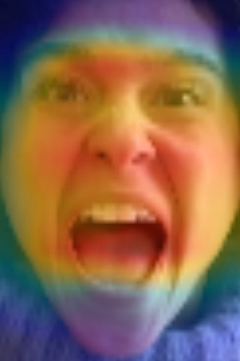
\includegraphics[scale=0.3]{figures/Layer_4_GradCAM.png}
    \end{subfigure}
    \hfill
    \begin{subfigure}{0.3\columnwidth}
        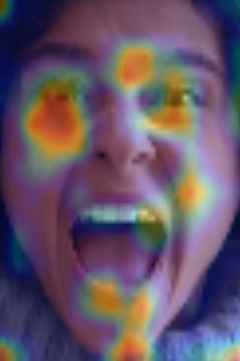
\includegraphics[scale=0.3]{figures/Layer_3_GradCAM.png}
    \end{subfigure}
    \hfill
    \begin{subfigure}{0.3\columnwidth}
        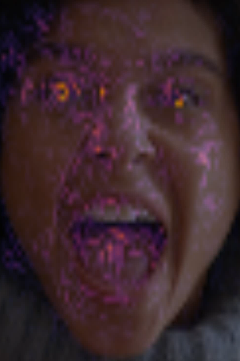
\includegraphics[scale=0.3]{figures/IntegratedGradients.png}
    \end{subfigure}
    \caption{Grad-CAM result of the fourth convolutional layer (left), the third convolutional layer (middle), and Integrated Gradients (right)}
    \label{fig:XAI}

\end{figure}

\subsubsection{Integrated gradients}

Integrated gradients is a different algorithm to assess the importance of different image regions for the model's decision. This method works by attributing importance values 
to the pixels of a baseline image. This image is slowly transformed into the original input image and in each transformation step the gradients of each pixel are calculated. The 
Importance of each pixel is then set as the average gradient of each pixel, which represents how much the model's output changes based on that piece of information \cite{DBLP:journals/corr/SundararajanTY17}.
The result is a fine grained attention map which highlights the most important parts of the image as seen in Figure \ref{fig:XAI}.

This approach seemed interesting to us as the quality of the output did not rely on the architectural details of our model.
